\documentclass{standalone}
\usepackage{tikz}
\usetikzlibrary{shapes.geometric}
\begin{document}
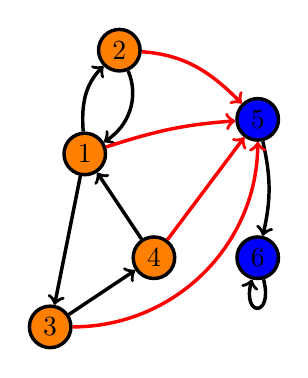
\begin{tikzpicture}
[every node/.style={inner sep=0pt}]
\node (1) [circle, minimum size=15.0pt, fill=orange, line width=1.25pt, draw=black] at (37.5pt, -62.5pt) {\textcolor{black}{1}};
\node (2) [circle, minimum size=15.0pt, fill=orange, line width=1.25pt, draw=black] at (50.0pt, -25.0pt) {\textcolor{black}{2}};
\node (4) [circle, minimum size=15.0pt, fill=orange, line width=1.25pt, draw=black] at (62.5pt, -100.0pt) {\textcolor{black}{4}};
\node (3) [circle, minimum size=15.0pt, fill=orange, line width=1.25pt, draw=black] at (25.0pt, -125.0pt) {\textcolor{black}{3}};
\node (6) [circle, minimum size=15.0pt, fill=blue, line width=1.25pt, draw=black] at (100.0pt, -100.0pt) {\textcolor{black}{6}};
\node (5) [circle, minimum size=15.0pt, fill=blue, line width=1.25pt, draw=black] at (100.0pt, -50.0pt) {\textcolor{black}{5}};
\draw [line width=1.25, ->, color=black] (1) to  (3);
\draw [line width=1.25, ->, color=black] (3) to  (4);
\draw [line width=1.25, ->, color=black] (4) to  (1);
\draw [line width=1.25, ->, color=black] (1) to  [in=225, out=94] (2);
\draw [line width=1.25, ->, color=black] (2) to  [in=32, out=293] (1);
\draw [line width=1.25, ->, color=black] (5) to  [in=77, out=283] (6);
\draw [line width=1.25, ->, color=black, loop below] (6) to (6);
\draw [line width=1.25, ->, color=red] (4) to  (5);
\draw [line width=1.25, ->, color=red] (1) to  [in=184, out=18] (5);
\draw [line width=1.25, ->, color=red] (2) to  [in=135, out=356] (5);
\draw [line width=1.25, ->, color=red] (3) to  [in=270, out=0] (5);
\end{tikzpicture}

\end{document}
